%!TEX TS-program = xelatex

% Шаблон документа LaTeX создан в 2018 году
% Алексеем Подчезерцевым
% В качестве исходных использованы шаблоны
% 	Данилом Фёдоровых (danil@fedorovykh.ru) 
%		https://www.writelatex.com/coursera/latex/5.2.2
%	LaTeX-шаблон для русской кандидатской диссертации и её автореферата.
%		https://github.com/AndreyAkinshin/Russian-Phd-LaTeX-Dissertation-Template

\documentclass[a4paper,14pt]{article}


%%% Работа с русским языком
\usepackage[english,russian]{babel}   %% загружает пакет многоязыковой вёрстки
\usepackage{fontspec}      %% подготавливает загрузку шрифтов Open Type, True Type и др.
\defaultfontfeatures{Ligatures={TeX},Renderer=Basic}  %% свойства шрифтов по умолчанию
\setmainfont[Ligatures={TeX,Historic}]{Times New Roman} %% задаёт основной шрифт документа
\setsansfont{Comic Sans MS}                    %% задаёт шрифт без засечек
\setmonofont{Courier New}
\usepackage{indentfirst}
\frenchspacing

\renewcommand{\epsilon}{\ensuremath{\varepsilon}}
\renewcommand{\phi}{\ensuremath{\varphi}}
\renewcommand{\kappa}{\ensuremath{\varkappa}}
\renewcommand{\le}{\ensuremath{\leqslant}}
\renewcommand{\leq}{\ensuremath{\leqslant}}
\renewcommand{\ge}{\ensuremath{\geqslant}}
\renewcommand{\geq}{\ensuremath{\geqslant}}
\renewcommand{\emptyset}{\varnothing}

%%% Дополнительная работа с математикой
\usepackage{amsmath,amsfonts,amssymb,amsthm,mathtools} % AMS
\usepackage{icomma} % "Умная" запятая: $0,2$ --- число, $0, 2$ --- перечисление

%% Номера формул
%\mathtoolsset{showonlyrefs=true} % Показывать номера только у тех формул, на которые есть \eqref{} в тексте.
%\usepackage{leqno} % Нумерация формул слева	

%% Перенос знаков в формулах (по Львовскому)
\newcommand*{\hm}[1]{#1\nobreak\discretionary{}
	{\hbox{$\mathsurround=0pt #1$}}{}}

%%% Работа с картинками
\usepackage{graphicx}  % Для вставки рисунков
\graphicspath{{images/}}  % папки с картинками
\setlength\fboxsep{3pt} % Отступ рамки \fbox{} от рисунка
\setlength\fboxrule{1pt} % Толщина линий рамки \fbox{}
\usepackage{wrapfig} % Обтекание рисунков текстом

%%% Работа с таблицами
\usepackage{array,tabularx,tabulary,booktabs} % Дополнительная работа с таблицами
\usepackage{longtable}  % Длинные таблицы
\usepackage{multirow} % Слияние строк в таблице
\usepackage{float}% http://ctan.org/pkg/float

%%% Программирование
\usepackage{etoolbox} % логические операторы


%%% Страница
\usepackage{extsizes} % Возможность сделать 14-й шрифт
\usepackage{geometry} % Простой способ задавать поля
\geometry{top=20mm}
\geometry{bottom=20mm}
\geometry{left=20mm}
\geometry{right=10mm}
%
%\usepackage{fancyhdr} % Колонтитулы
% 	\pagestyle{fancy}
%\renewcommand{\headrulewidth}{0pt}  % Толщина линейки, отчеркивающей верхний колонтитул
% 	\lfoot{Нижний левый}
% 	\rfoot{Нижний правый}
% 	\rhead{Верхний правый}
% 	\chead{Верхний в центре}
% 	\lhead{Верхний левый}
%	\cfoot{Нижний в центре} % По умолчанию здесь номер страницы

\usepackage{setspace} % Интерлиньяж
\onehalfspacing % Интерлиньяж 1.5
%\doublespacing % Интерлиньяж 2
%\singlespacing % Интерлиньяж 1

\usepackage{lastpage} % Узнать, сколько всего страниц в документе.

\usepackage{soul} % Модификаторы начертания

\usepackage{hyperref}
\usepackage[usenames,dvipsnames,svgnames,table,rgb]{xcolor}
\hypersetup{				% Гиперссылки
	unicode=true,           % русские буквы в раздела PDF
	pdftitle={Автоматизация проектных работ},   % Заголовок
	pdfauthor={Солодянкин А.А.},      % Автор
	pdfsubject={Автоматизация проектных работ},      % Тема
	pdfcreator={Солодянкин А.А.}, % Создатель
	pdfproducer={Солодянкин А.А.}, % Производитель
	pdfkeywords={Автоматизация проектных работ}, % Ключевые слова
	colorlinks=true,       	% false: ссылки в рамках; true: цветные ссылки
	linkcolor=black,          % внутренние ссылки
	citecolor=black,        % на библиографию
	filecolor=magenta,      % на файлы
	urlcolor=black           % на URL
}
\makeatletter 
\def\@biblabel#1{#1. } 
\makeatother
\usepackage{cite} % Работа с библиографией
%\usepackage[superscript]{cite} % Ссылки в верхних индексах
%\usepackage[nocompress]{cite} % 
\usepackage{csquotes} % Еще инструменты для ссылок

\usepackage{multicol} % Несколько колонок

\usepackage{tikz} % Работа с графикой
\usepackage{pgfplots}
\usepackage{pgfplotstable}

% ГОСТ заголовки
\usepackage[font=small]{caption}
%\captionsetup[table]{justification=centering, labelsep = newline} % Таблицы по правобу краю
%\captionsetup[figure]{justification=centering} % Картинки по центру


\newcommand{\tablecaption}[1]{\addtocounter{table}{1}\small \begin{flushright}\tablename \ \thetable\end{flushright}%	
\begin{center}#1\end{center}}

\newcommand{\imref}[1]{рис.~\ref{#1}}

\usepackage{multirow}
\usepackage{spreadtab}
\newcolumntype{K}[1]{@{}>{\centering\arraybackslash}p{#1cm}@{}}


\usepackage{xparse}
\usepackage{fancyvrb}

\RecustomVerbatimCommand{\VerbatimInput}{VerbatimInput}
{
	fontsize=\footnotesize    
}

\newcolumntype{?}[1]{!{\vrule width #1}}

\usepackage{tocloft}
\renewcommand{\cftsecleader}{\cftdotfill{\cftdotsep}}
\begin{document} % конец преамбулы, начало документа
\begin{titlepage}
	\begin{center}
		ПРАВИТЕЛЬСТВО РОССИЙСКОЙ ФЕДЕРАЦИИ \\
 		ФЕДЕРАЛЬНОЕ  ГОСУДАРСТВЕННОЕ АВТОНОМНОЕ \\
		ОБРАЗОВАТЕЛЬНОЕ УЧРЕЖДЕНИЕ ВЫСШЕГО ОБРАЗОВАНИЯ\\
		«НАЦИОНАЛЬНЫЙ ИССЛЕДОВАТЕЛЬСКИЙ УНИВЕРСИТЕТ\\
		«ВЫСШАЯ ШКОЛА ЭКОНОМИКИ»
	\end{center}
	
	\begin{center}
		\textbf{Московский институт электроники и математики}
		
		\textbf{Им. А.Н.Тихонова НИУ ВШЭ}
		
		\vspace{2ex}
		
		\textbf{Департамент компьютерной инженерии}
	\end{center}
	\vspace{1ex}	
	
	\vspace{1ex}
	\begin{center}
		\textbf{Практическая работа №5 \\
			«Разработка конвейерного умножителя в среде Altera Quartus II» \\
			Вариант №13
	}
	\end{center}	

	\vspace{2ex}
	\vfill
	
	\vspace{2ex}
	
	\begin{flushright}
		\textbf{Выполнил:}
		
		\vspace{2ex}
		
		Студент группы БИВ174
		
		\vspace{2ex}
		
		Солодянкин Андрей Александрович
		
		\vspace{2ex}
		
		\textbf{Проверил:}
		
		\vspace{2ex}
		
		Романова Ирина Ивановна
	\end{flushright}

	\vspace{5ex}
	\begin{center}
		Москва \the\year \, г.
	\end{center}
	
\end{titlepage}
\addtocounter{page}{1}

\tableofcontents
\pagebreak

\section{Цель работы}

Моделирование работы дешифратора, изучение карт Карно.

\section{Задание}

\begin{enumerate}
\item Выполнить действия, описанный в практической работе 5 -- Часть 1, 2, 3;

\item Оформить отчет, который должен включать: титульный лист, введение и постановку задачи, тему работы, описание всех этапов выполнения проекта, скриншоты (рисунки с подрисуночными подписями) ключевых моментов, выводы;

\item Изменить схему устройства добавив собственный блок памяти.
Объяснить работу устройства;

\item Изменить схему устройства добавив арифметический блок.
Объяснить работу устройства.

\end{enumerate}

\section{Часть 1. «Знакомство со средой проектирования Quartus II. Создание проекта»}

\subsection{Создание проекта}

Для начала необходимо открыть Quartus, открываем его.

Далее заходим в меню File и выбираем New Project Wizard.
В открывшемся окне жмем Next, в следующем выбираем директорию для проекта и вводим имя проекта, жмем 2 раза Next.

В следующем окне выбираем все как на рис. \ref{fig:screenshot42} и жмем далее 2 раза.

\begin{figure}[H]
	\centering
	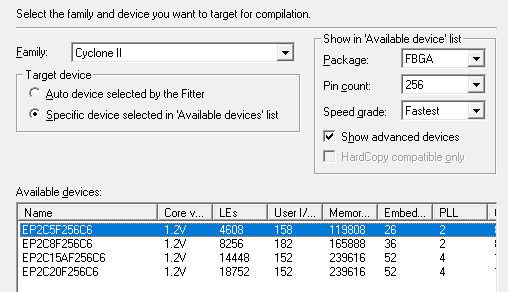
\includegraphics[width=0.7\linewidth]{image/lab5/Screenshot_42}
	\caption{Создание нового проекта}
	\label{fig:screenshot42}
\end{figure}

На последнем шаге должны получится значения как на рис. \ref{fig:screenshot43}.

\begin{figure}[H]
	\centering
	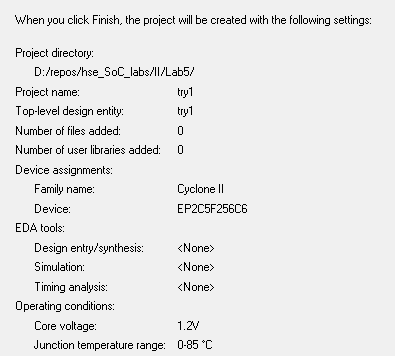
\includegraphics[width=0.7\linewidth]{image/lab5/Screenshot_43}
	\caption{}
	\label{fig:screenshot43}
\end{figure}

\subsection{Разработка конвейерного умножителя}

\subsubsection{Создание умножителя 8х8 с помощью утилиты Mega Wizard\textregistered  Plug-in Manager}

Для создания необходимо в меню выбрать Tools > Mega Wizard  Plug-in Manager, в открывшемся окне выбираем опцию Create a new custom megafunction variation. Далее в папке Arithmetics выбираем LPM\_MULT (рис. \ref{fig:screenshot412}). Семейство микросхем выбираем Cyclone II.

\begin{figure}[H]
	\centering
	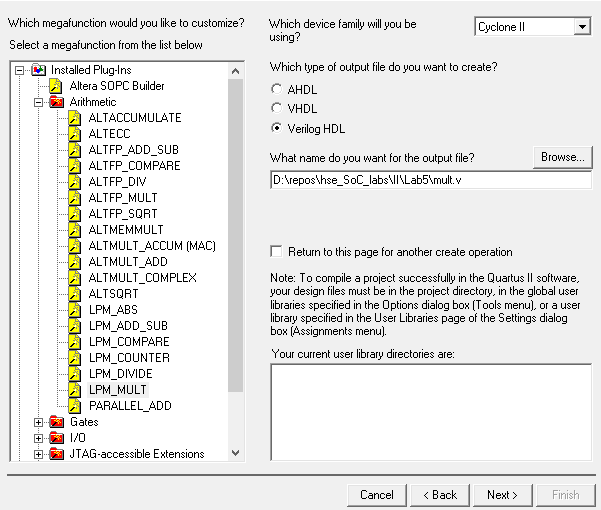
\includegraphics[width=0.7\linewidth]{image/lab5/Screenshot_412}
	\caption{Создание мегафункции}
	\label{fig:screenshot412}
\end{figure}

Поля dataa и datab на рис. \ref{fig:screenshot002} оставляем по 8 бит. Жмем next 2 раза.

\begin{figure}[H]
	\centering
	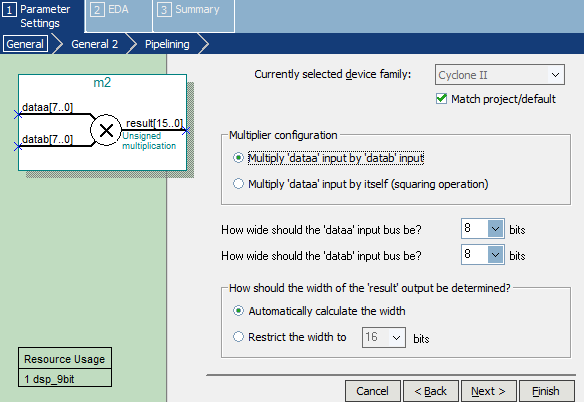
\includegraphics[width=0.7\linewidth]{image/lab5/screenshot002}
	\caption{Создание мегафункци}
	\label{fig:screenshot002}
\end{figure}

Далее в первом окне выбираем yes и вводим число 2 (рис. \ref{fig:screenshot003}), нажимаем next 2 раза.

\begin{figure}[H]
	\centering
	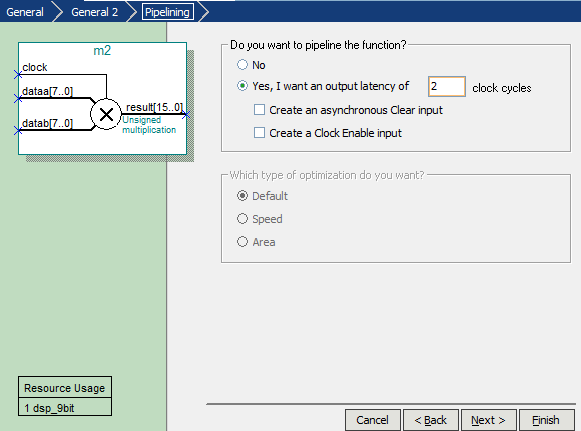
\includegraphics[width=0.7\linewidth]{image/lab5/screenshot003}
	\caption{Создание мегафункци}
	\label{fig:screenshot003}
\end{figure}

На текущем окне (рис. \ref{fig:screenshot423}) выбираем все в соответствии с рисунком и жмем на finish. После этого мегафункция готова.

\begin{figure}[H]
	\centering
	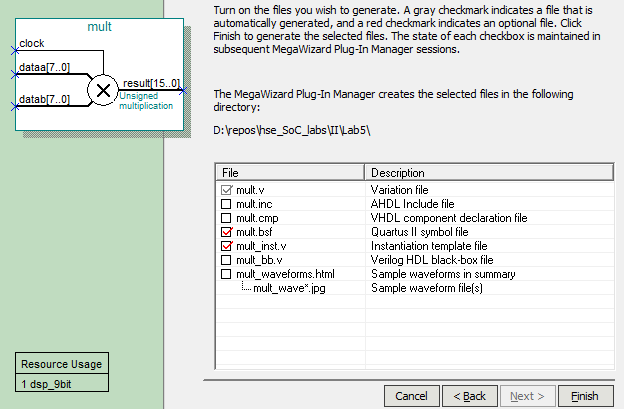
\includegraphics[width=0.7\linewidth]{image/lab5/Screenshot_423}
	\caption{Создание мегафункци}
	\label{fig:screenshot423}
\end{figure}

\subsubsection{Создание 32х16 RAM с помощью утилиты Mega Wizard\textregistered  Plug-in Manager}

Для создания необходимо в меню выбрать Tools > Mega Wizard  Plug-in Manager, в открывшемся окне выбираем опцию Create a new custom megafunction variation. Далее в папке Memory Compiler выбираем RAM: 2-PORT (рис. \ref{fig:screenshot004}). Семейство микросхем выбираем Cyclone II.

\begin{figure}[H]
	\centering
	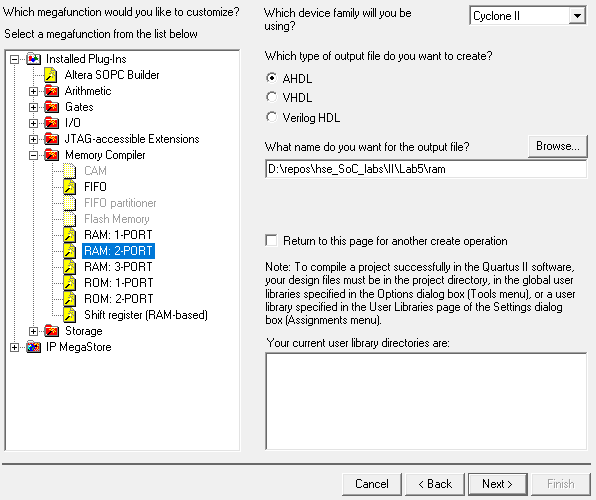
\includegraphics[width=0.7\linewidth]{image/lab5/screenshot004}
	\caption{Создание мегафункци RAM}
	\label{fig:screenshot004}
\end{figure}

На следующей странице ничего не нажимаем, жмем только на next.

На странице Widths/Blk Type необходимо установить разрядность входного порта data\_a 16 bit (рис. \ref{fig:screenshot005}). После этого жмем Next 2 раза.

\begin{figure}[H]
	\centering
	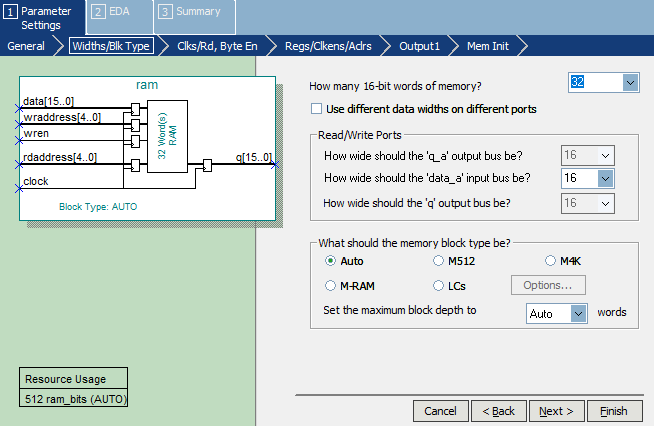
\includegraphics[width=0.7\linewidth]{image/lab5/screenshot005}
	\caption{Создание мегафункци RAM}
	\label{fig:screenshot005}
\end{figure}

На странице Regs/Clkens/Aclrs отключем опцию Read output port(s) 'q' (рис. \ref{fig:screenshot006}). Больше ничего не трогаем, жмем Next 2 раза.

\begin{figure}[H]
	\centering
	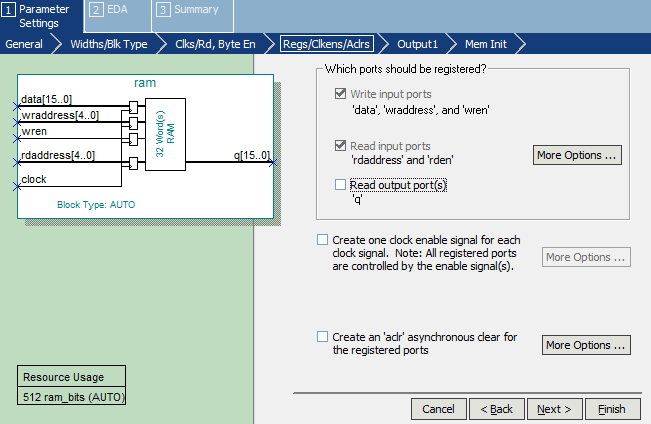
\includegraphics[width=0.7\linewidth]{image/lab5/screenshot006}
	\caption{Создание мегафункци RAM}
	\label{fig:screenshot006}
\end{figure}

На странице Mem Init выбираем yes и указываем имя файла ram.hex (рис. \ref{fig:screenshot007}). После этого жмем Next.

\begin{figure}[H]
	\centering
	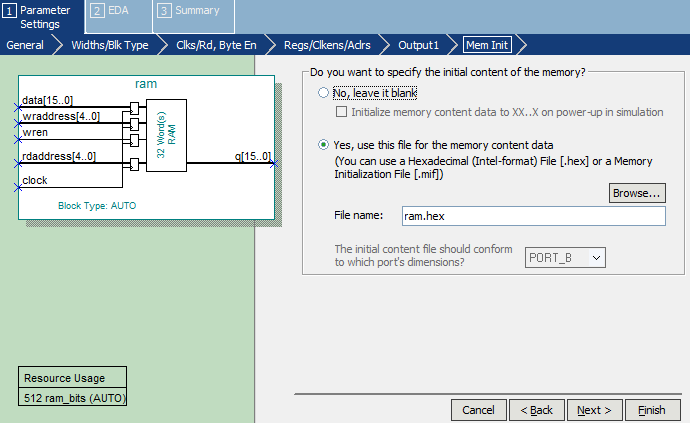
\includegraphics[width=0.7\linewidth]{image/lab5/screenshot007}
	\caption{Создание мегафункци RAM}
	\label{fig:screenshot007}
\end{figure}

Последние шаги совпадают с шагами для создания умножителя.

\subsubsection{Создание HEX файл с помощью редактора Memory Editor}

Вменю File выбираем команду New, в открывшемся окне выбираем Other Files и выбираем Hexadecimal (Intel-Format) File. В открытом окне вводим 32 и 16.

\begin{figure}[H]
	\centering
	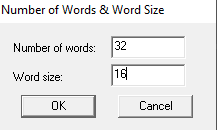
\includegraphics[width=0.4\linewidth]{image/lab5/screenshot008}
	\caption{Создание HEX файла}
	\label{fig:screenshot008}
\end{figure}

Получаем следующий файл рис. \ref{fig:screenshot009}

\begin{figure}[H]
	\centering
	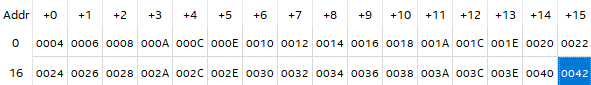
\includegraphics[width=0.7\linewidth]{image/lab5/screenshot012}
	\caption{HEX файл}
	\label{fig:screenshot012}
\end{figure}


Заполняем файл при помощи функции Custom Fill Cells.

\subsubsection{Добавление блоков в проект и создание связей}

Создаем схему и подтягиваем туда созданные ранее мегафункции (рис. \ref{fig:screenshot011}).

\begin{figure}[H]
	\centering
	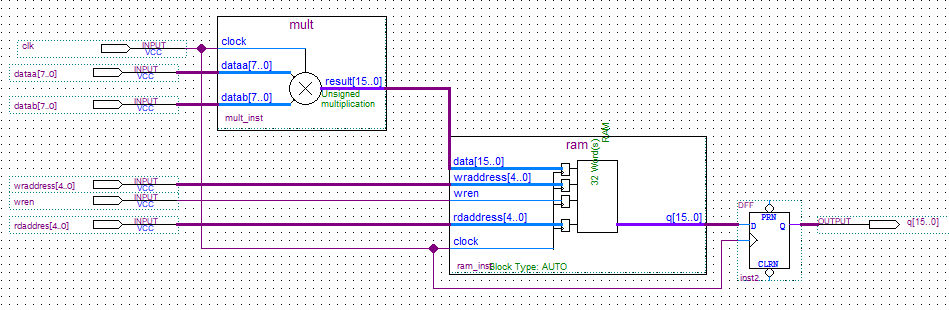
\includegraphics[width=0.8\linewidth]{image/lab5/screenshot011}
	\caption{Итоговая схема}
	\label{fig:screenshot011}
\end{figure}

\section{Часть 2. «Моделирование проекта в среде Quartus II»}

Создадим модуляцию проекта при помощи University Program VWF. 

Добавим пины: clk, wren, data, datab, rdaddres, wraddres, q.

\begin{figure}[H]
	\centering
	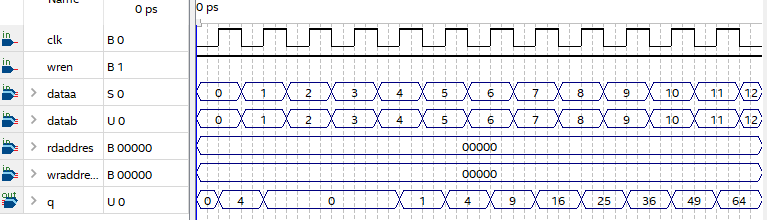
\includegraphics[width=0.9\linewidth]{image/lab5/screenshot013}
	\caption{Результат модуляции проекта}
	\label{fig:screenshot013}
\end{figure}

\section{Часть 3. «Компиляция проекта в среде Quartus II. Анализ результатов компиляции»}

\subsection{Компиляция проекта}

Скомпилируем проект, результат компиляции  представлен на рис. \ref{fig:screenshot014}.

\begin{figure}[H]
	\centering
	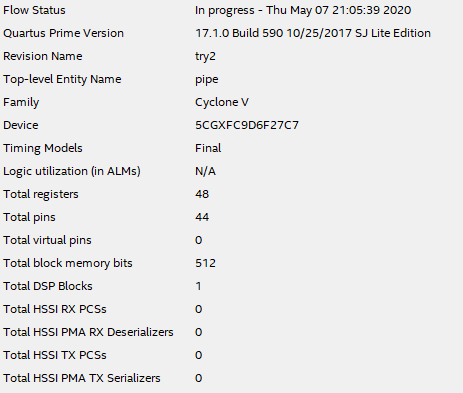
\includegraphics[width=0.7\linewidth]{image/lab5/screenshot014}
	\caption{Результаты компиляции проекта}
	\label{fig:screenshot014}
\end{figure}

\subsection{RTL представление проекта}

На рис. \ref{fig:screenshot015} RTL представление проекта.

\begin{figure}[H]
	\centering
	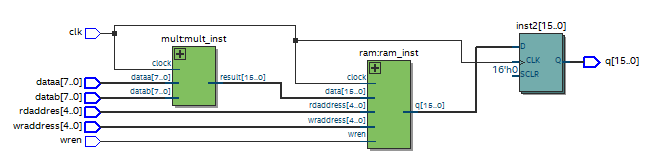
\includegraphics[width=0.7\linewidth]{image/lab5/screenshot015}
	\caption{RTL представление}
	\label{fig:screenshot015}
\end{figure}

Внутренности ram (рис. \ref{fig:screenshot016}), внутри он состоит из 16 однобитных регистров.

\begin{figure}[H]
	\centering
	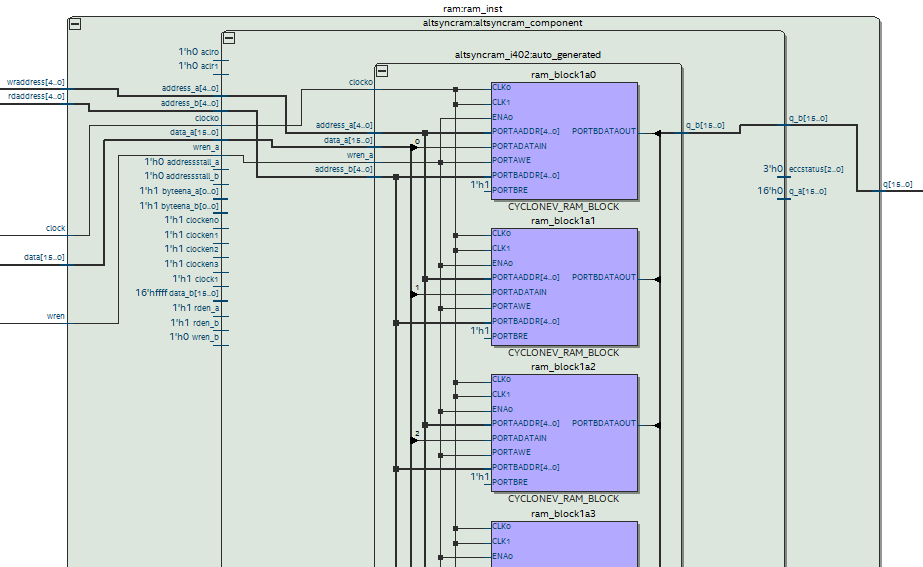
\includegraphics[width=0.7\linewidth]{image/lab5/screenshot016}
	\caption{Внутренности ram}
	\label{fig:screenshot016}
\end{figure}

\subsection{Редактор chip planner}

Нажмем правой кнопкой на элемент однобитного элемента ram, далее Locate Node -> Locate in Chip planner. 
Результат представлен на рис. \ref{fig:screenshot017}.

\begin{figure}[H]
	\centering
	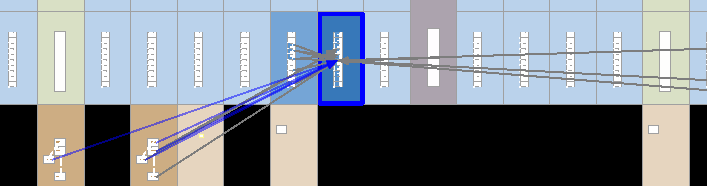
\includegraphics[width=0.7\linewidth]{image/lab5/screenshot017}
	\caption{Отображение связей элемента}
	\label{fig:screenshot017}
\end{figure}

\section{Доп задание}

Изменим схему, вместо первого числа поставим счетчик, а вместо двухпортовой памяти поставим однопортовую (рис. \ref{fig:screenshot018}).

\begin{figure}[H]
	\centering
	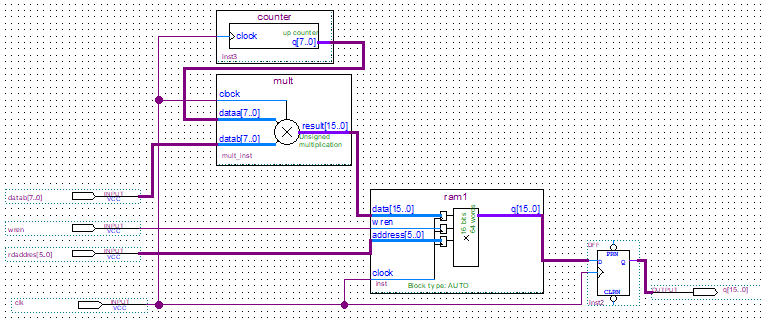
\includegraphics[width=0.7\linewidth]{image/lab5/screenshot018}
	\caption{Блок схема доп задания}
	\label{fig:screenshot018}
\end{figure}

Результаты компиляции проекта (рис. \ref{fig:screenshot021})

\begin{figure}[H]
	\centering
	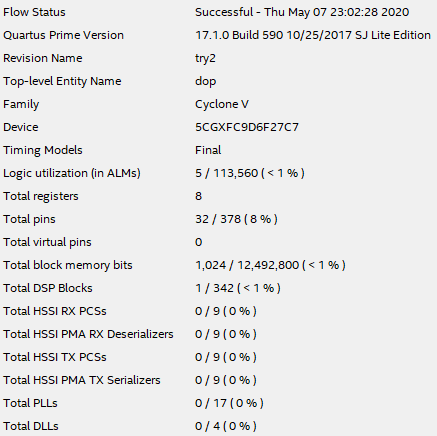
\includegraphics[width=0.7\linewidth]{image/lab5/screenshot021}
	\caption{Результат компиляции доп задания}
	\label{fig:screenshot021}
\end{figure}


Временная диаграмма доп задания (рис. \ref{fig:screenshot019}).

\begin{figure}[H]
	\centering
	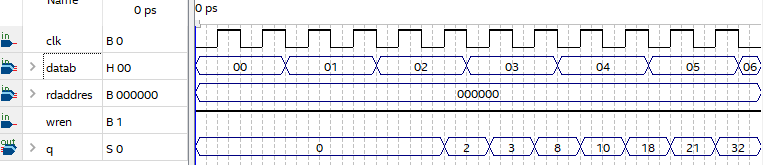
\includegraphics[width=0.7\linewidth]{image/lab5/screenshot019}
	\caption{WVF диаграмма}
	\label{fig:screenshot019}
\end{figure}

RTL представление доп задания (рис. \ref{fig:screenshot020}).

\begin{figure}[H]
	\centering
	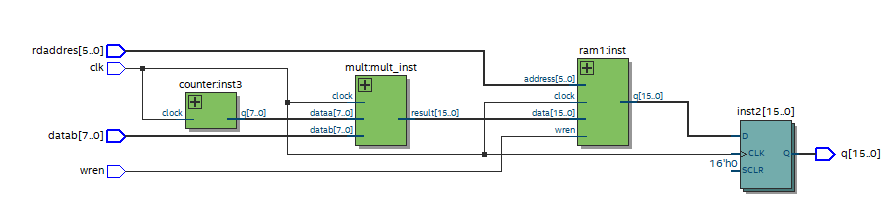
\includegraphics[width=0.7\linewidth]{image/lab5/screenshot020}
	\caption{RTL представление}
	\label{fig:screenshot020}
\end{figure}

Связи на Chip Planner (рис. \ref{fig:screenshot022}).

\begin{figure}[H]
	\centering
	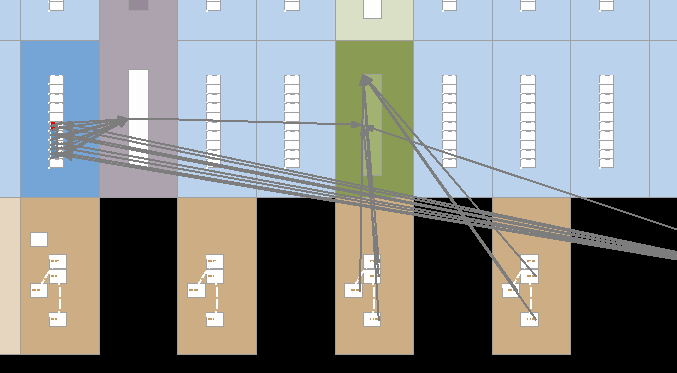
\includegraphics[width=0.7\linewidth]{image/lab5/screenshot022}
	\caption{Отображение связей элемента}
	\label{fig:screenshot022}
\end{figure}


\section{Вывод}
В ходе проделанной работы было создано 2 проекта арифметических устройств с памятью.

Были созданы мегафункции умножителя, счетчика одно- и дву- портовые элементы памяти при помощи Mega Wizard  Plug-in Manager.

Схема была протестированы при помощи WaveForm, были рассмотрены схемы, полученные при помощи Chip planner.
\newpage 
\renewcommand{\refname}{{\normalsize СПИСОК ИСПОЛЬЗОВАННЫХ ИСТОЧНИКОВ}} 
\centering 
\begin{thebibliography}{9} 
	\addcontentsline{toc}{section}{\refname} 
	\bibitem{sql} Vijayakumar P., Vijayalakshmi V., Zayaraz G. Comparative study of hyperelliptic curve cryptosystem over prime field and its survey //International Journal of Hybrid Information Technology. – 2014. – Т. 7. – №. 1. – С. 137-146.
	\bibitem{sql} Антонов А., Филиппов А., Золотухо Р. Средства системной отладки САПР Quartus II //Компоненты и технологии. – 2008. – №. 89.
\end{thebibliography}

\end{document} % конец документа